\documentclass{article}
\usepackage{amsmath, amssymb, mathtools, verbatim, tikz, graphicx,nicefrac}
\usepackage[margin=0.5in]{geometry}
\graphicspath{{images/}}
\setlength{\parindent}{0pt}
\renewcommand{\t}[1]{\text{#1}}
\newcommand{\N}{\mathbb{N}}
\newcommand{\sumx}[2]{\sum\limits_{#1}^{#2}}
\newcommand{\ord}{\text{ord}}
\newcommand{\frp}{\text{FRP}}
\newcommand{\R}{\Rightarrow\,}
\newcommand{\B}[1]{\textbf{#1}}
\newcommand{\I}[1]{\textit{#1}}
\newcommand{\U}{\bigcup}
\newcommand{\V}{\vert}
\newcommand{\F}[1]{\lfloor#1\rfloor}
\newcommand{\T}[1]{\text{#1}}
\newcommand{\lra}[1]{\langle#1\rangle}
\newcommand{\len}[1]{\vert#1\vert}
\newcommand{\num}{\text{num}}
\newcommand{\nfrc}[2]{\nicefrac{#1}{#2}}
\newcommand{\nim}{\mathcal{N}}
\newcommand{\xor}{\oplus}
\newcommand{\D}[2]{D_{#1}^{#2}}
\newcommand{\SUDL}{single-up double-left}
\newcommand{\DUSL}{double-up single-left}
\newenvironment{claim}[1]{\par\noindent\underline{Claim:}\space#1}{}
\newenvironment{claimproof}[1]{\par\noindent\underline{Proof:}\space#1}
{\hfill $\blacksquare$}
\newcommand{\game}[3]{\begin{array}{@{}*6r}(#1, & #2, & #3)\end{array}}
\newcommand{\gcong}{\cong\:}
\begin{document}
\begin{center}
  21--499 Report, Kartik Sabharwal (ksabharw) \\
\end{center}
\paragraph{Bowling Description}\mbox{}\\
Two people --- we'll call them $A$ and $B$ --- are playing a bowling game. \\
They have $n$ bowling pins in a row, and they take turns to knock over
pins using special bowling balls until there are no pins left standing. \\
The first bowling ball is \textit{small}, and it always knocks over
just one pin. \\
The other one is \textit{large}, and it always knocks over exactly 3 pins. To
be clear, a player is only allowed to use a large ball on three pins
that are right next to each other. \\
No player ever misses. \\
$A$ goes first, and if a player has no available moves in her turn
(i.e.\ if the player that went before knocked over all the pins) then she
loses.
\bigskip

\paragraph{Bowling Analysis}\mbox{}\\
Our goal is to find the nimber for any $n$-size row of starting pins. \\
Let the function mapping $n$ to its nimber be $\nim$. \\
Also, number the pins 1, 2, $\ldots$, $n$ from left to right.
\bigskip

\begin{claim}
\begin{equation*}
  \nim(n) =
  \begin{cases}
    1,\ \T{if}\ n\ \T{is odd} \\
    0,\ \T{if}\ n\ \T{is even}
  \end{cases}
\end{equation*}
\end{claim}

\begin{claimproof}\mbox{}\\
  We will prove this by strong induction.
  \medskip

  \I{Base Cases:} \\
  $\nim(0) = 0$ \\
  $\nim(1) = 1$ \\
  $\nim(2) = 0$ \\
  $\nim(3) = 1$ \\
  Thus, the claim holds for $n = 0, 1, 2$ or $3$.
  \medskip

  \I{Induction Hypothesis:} \\
  Suppose for some $m \geq 4$, the claim is true for all $i < m$.
  \medskip

  \I{Induction Step:} \\
  We want to prove that the claim is true for $m + 1$.
  \smallskip

  If $m + 1$ is odd, then throwing a large bowling ball will
  reduce the number of pins to $m - 2$, and throwing a small
  bowling ball will reduce the number of pins to $m$. Notice
  that both $m$ and $m - 2$ must be even numbers. To sum up,
  throwing any bowling ball will give us an even number of
  pins. \\
  If the pins knocked over are all on either the left or right
  end of the row, then we will be left with a continuous row
  of an even number of pins. By the I.H.\ such a position has
  nimber $0$. \\
  If the pins knocked over are somewhere in the middle of the row,
  we will be left with two continuous rows of pins, with a
  ``gap'' in the middle that was formerly occupied by the
  knocked pins. These two continuous rows must either both have
  an even number of pins or both have an odd number of pins.
  In the former case, the situation will have nimber $0 \xor 0 = 0$
  and in the latter case, the situation will have nimber $1 \xor 1 = 0$. \\
  It follows that all the ``child'' positions of the situation with
  a row of $m + 1$ pins have nimber $0$. So, the minimum excluded
  value is $1$, which means $\nim(m + 1) = 1$ when $m + 1$ is odd. 
  \smallskip

  If $m + 1$ is even, then throwing a large bowling ball will
  reduce the number of pins to $m - 2$, and throwing a small
  bowling ball will reduce the number of pins to $m$. Notice
  that both $m$ and $m - 2$ must now be odd numbers. To sum up,
  throwing any bowling ball will give us an odd number of
  pins. \\
  If the pins knocked over are all on either the left or right
  end of the row, then we will be left with a continuous row
  of an odd number of pins. By the I.H.\ such a position has
  nimber $1$. \\
  If the pins knocked over are somewhere in the middle of the row,
  we will be left with two continuous rows of pins, with a
  ``gap'' in the middle that was formerly occupied by the
  knocked pins. One of these rows must have an even number of pins
  and the other row must have an odd number of pins. By the
  I.H.\ in this situation the nimber is either $0 \xor 1 = 1$
  or $1 \xor 0 = 1$. \\
  It follows that all the ``child'' positions of the situation with
  a row of $m + 1$ pins have nimber $1$. So, the minimum excluded
  value is $0$, which means $\nim(m + 1) = 0$ when $m + 1$ is even. 
  \smallskip

  We have proved the claim to be true for $m + 1$. \\
  Thus by strong induction the claim must hold for all natural
  numbers.
\end{claimproof}
\newpage

\paragraph{Bowling Possibilities}\mbox{}\\
Suppose the rule about the use of the \I{large} bowling ball
is altered, and now players can disregard ``gaps'' in the row
of pins while throwing the large ball. \\
To illustrate, in the previous game if a player was faced with
the following situation (each vertical line represents a pin, and
each star represents a position in the row previously occupied by
a pin but now empty):
\begin{verbatim}
  | | * | | |
\end{verbatim}
then the players would have to treat it as two ``disjoint'' piles. \\
Now, they are allowed to throw a large ball in such a way that
they can turn the above position to the following one in a single
move:
\begin{verbatim}
  | * * * | |
\end{verbatim}
One might ask how this changes the nimbers that can be achieved. The
answer is that it makes things much less well-behaved. The nimbers
from $n = 0$ to $n = 100$, in array form, are:
\begin{verbatim}
rawNimbers = [ 0, 0, 1, 0, 0, 0, 1, 2, 3, 0, 
               0, 0, 0, 0, 9, 2, 8, 0, 0, 0, 
               0, 1,15, 1, 0, 0, 0, 1,11,10, 
               0, 0, 0, 0, 0,22, 1,20, 0, 0, 
               0, 0, 0, 0,29, 1, 8, 0, 0, 0, 
               5, 1,10, 0, 0, 0,21, 2, 9, 0, 
               0, 0, 0, 0, 0,39,10,11, 0, 0, 
               0, 0, 1,17,10, 0, 0, 0, 1,16,
               9, 0, 0, 0, 0, 0,10, 1,40, 0,
               0, 0, 0,22,18, 8, 0, 0, 0, 9,
               67 ]
\end{verbatim}
We can plot with $n$ on the $x$-axis versus $\nim(n)$ on the y-axis to get:
\begin{center}
  \includegraphics[scale=0.7]{bowlingScatter}
\end{center}
I looked at the nimbers, as well as the differences between these
nimbers, and there were no good, reliable patterns. I tried to prove
first that there was no upper bound on the nimbers as $n$ increases,
and also that there are infinitely many $0$-positions, but I could not
get that to work. \\
Furthermore, I believe that more data is necessary to see if this
eventually becomes periodic or not, but even after spending a considerable
amount of time memoizing and optimizing my code, computing nimbers
for $n$ higher than 100 did not take viable amounts of time. \\
I moved to a new game, which I will discuss in the next section.
\newpage

\paragraph{Transfer Description}\mbox{}\\
This is a game for two players, who take turns making moves. \\
We have three points $\mathbb{P} = \{P_1, P_2, P_3\}$ in a plane. \\
Consider a function $s : \mathbb{P} \rightarrow \N$, where
$s(P_i)$ denotes the number of ``stones'' at point $P_i$. \\
Initially, $s(P_1) = s(P_3) = 0$ and $s(P_2) = n$. \\
A player, in her turn, may either move some stones from
$P_2$ to $P_1$ or she may move some stones from $P_2$ to $P_3$,
but she can't do both. \\
Also, the following invariants must be respected:
\begin{enumerate}
  \item $s(P_1) \leq s(P_2)$ and $s(P_3) \leq s(P_2)$.
  \item If, at the start of a player's turn, $s(P_1) < s(P_3)$ then
    at the end of the turn $s(P_1) \leq s(P_3)$ must hold. \\
    Similarly, if at the start of a player's turn it is true that
    $s(P_3) < s(P_1)$ then at the end of the turn
    $s(P_3) \leq s(P_1)$ must hold.
\end{enumerate}
If a player cannot make any moves, then she loses. \\
This means we can describe a game of this form with a tuple
$\game{a}{b}{c}$ which means $s(P_1) = a, s(P_2) = b, s(P_3) = c$. \\

\paragraph{Transfer Analysis}\mbox{}\\
We claim that:
\begin{equation*}
  \nim\game{0}{n}{0} =
  \begin{cases}
    0, & \ \T{if}\ n \ \T{is odd or} n = 0 \\
    1, & \ \T{if}\ n \ \T{is even and}\ n \neq 4 \\
    2, & \ \T{if}\ n = 4
  \end{cases}
\end{equation*}

We can easily find out that: \\
$\nim\game{0}{0}{0} = 0$ \\
$\nim\game{0}{1}{0} = 1$ \\
$\nim\game{0}{2}{0} = 0$ \\
$\nim\game{0}{3}{0} = 1$ \\
$\nim\game{0}{4}{0} = 2$ \\
$\nim\game{0}{5}{0} = 1$
\bigskip

Then, we prove all the following for $n \geq 0$: \\
$\nim\game{0}{6n+6}{0} = 0$ \\
$\nim\game{0}{6n+7}{0} = 1$ \\
$\nim\game{0}{6n+8}{0} = 0$ \\
$\nim\game{0}{6n+9}{0} = 1$ \\
$\nim\game{0}{6n+10}{0} = 0$ \\
$\nim\game{0}{6n+11}{0} = 1$
\bigskip

Each of the proofs involves casing on whether the number of
stones moved by the first player is
$< \frac{6n+i}{3}$ and even, $< \frac{6n+i}{3}$ and odd, or
just $\geq \frac{6n+i}{3}$.
\bigskip

Note that we provide a full induction proof for the
$\game{0}{6n+8}{0}$ case, and for the others we show exactly how
to modify the first proof to give us the needed result.
\newpage

\paragraph{Proof for $6n + 8$ Case}\mbox{}\\
We want to prove the following proposition:
\begin{equation*}
  P(n) : \game{0}{6n + 8}{0} \gcong *1 \enspace \text{where} \enspace n \geq 0
\end{equation*}
We will use strong induction to prove the above statement.

\bigskip
\textbf{Base Cases:} \\
Using our program, we have verified that $P(n)$ holds for
$n \in \{0, 1, 2, 3\}$. \\
The fact that $\game{0}{2}{0} \gcong *1$ will also be useful.

\bigskip
\textbf{Induction Hypothesis:} \\
Assume for some $k \geq 1$ that 
$\forall \: n < k, \: P(n) \: \text{holds}$.

\bigskip
\textbf{Induction Step:} \\
We need to prove that $P(k)$ holds. In other words, we need to show:
\begin{equation*}
  \game{0}{6k + 8}{0} \gcong *1
\end{equation*}

\bigskip
\textit{Simplifying the problem,}\\
To show that $\game{0}{6k+8}{0}$ has nimber $1$, it suffices to show
the following:
\begin{enumerate}
  \item In one move, we can reach a state with nimber $0$
  \item In one move, we cannot reach a state with nimber $1$
\end{enumerate}

\bigskip
\textit{Looking at the initial state's children,}\\
Notice that in one move from the original state we can reach any state
of the form:
\begin{equation*}
  \game{m}{6k+8-m}{0} \text{where} \: 1 \leq m \leq 3k + 4 
  \end{equation*}
the remaining states that we can reach from the original state are of
the form:
\begin{equation*}
  \game{0}{6k+8-m}{m} \text{where} \: 1 \leq m \leq 3k + 4
\end{equation*}
Since the latter form is symmetric to the former, focusing our analysis
on the former is enough to complete the proof.

\bigskip
\textit{When} $m = 3k + 4$:\\
Observe that when $m = 3k + 4$, we obtain the state
$\game{3k+4}{3k+4}{0}$ which clearly has nimber $0$,
so we have proved the first fact we need. \\

\bigskip
\textit{When} $m$ \textit{is odd and} $1 \leq m \leq 2k + 2$:\\
When $m$ is an odd number satisfying $1 \leq m \leq 2k + 2$,
notice that
\begin{equation*}
  \game{m+1}{3k+4-\frac{m+1}{2}}{3k+4-\frac{m+1}{2}} \gcong *0
\end{equation*}
Work one step backwards from this to get
\begin{equation*}
  \game{m}{3k+5-\frac{m+1}{2}}{3k+4-\frac{m+1}{2}} \gcong *1
\end{equation*}
Observe that
\begin{equation*}
  \game{m}{6k+8-m}{0} \xrightarrow{\text{one move}}
  \game{m}{3k+5-\frac{m+1}{2}}{3k+4-\frac{m+1}{2}}
\end{equation*}
It follows that the minimum excluded value of the nimbers of
all the child states of $\game{m}{6k+8-m}{0}$ cannot be $1$, and
thus the nimber of this state cannot be 1, by the Sprague-Grundy
theorem.

\newpage
\textit{When} $m$ \textit{is even and} $1 \leq m \leq 2k + 2$:\\
When $m$ is an even number satisfying $1 \leq m \leq 2k + 2$,
observe that 
\begin{equation*}
  \game{m}{6k+8-m}{0} \xrightarrow{\text{one move}}
  \game{m}{6k+8-2m}{m}
\end{equation*}
We can replace $m$ with $2i$ where $1 \leq i \leq k + 1$ to get
\begin{equation*}
  \game{2i}{6k+8-2i}{0} \xrightarrow{\text{one move}}
  \game{2i}{6k+8-4i}{2i}
\end{equation*}
In the resultant state, the difference between the left and middle
values, also the difference between the right and middle values, is
\begin{equation*}
  6(k - i) + 8
\end{equation*}
Which intuitively suggests that
\begin{equation*}
  \game{2i}{6k+8-4i}{2i} \gcong \game{0}{6(k - i) + 8}{0} \:
  \text{for $1 \leq i \leq k + 1$}
\end{equation*}
and although we lack a rigorous argument for this we will assume it is
true. \\
Our knowledge that $\game{0}{2}{0} \gcong *1$ and also our induction
hypothesis, tell us:
\begin{equation*}
  \game{0}{6(k - i) + 8}{0} \gcong *1 \:
  \text{for $1 \leq i \leq k + 1$}
\end{equation*}
Consequently, $\game{2i}{6k+8-4i}{2i} \gcong *1$. \\
It follows that the minimum excluded value of the nimbers of
all the child states of $\game{m}{6k+8-m}{0}$ cannot be $1$, and
thus the nimber of this state cannot be 1.

\bigskip
\textit{When} $m \geq 2k + 3$:\\
If $m \geq 2k + 3$, it is clear that
\begin{equation*}
  \game{m}{m}{6k+8-2m} \gcong *0
\end{equation*}
Working backwards from this, we get that
\begin{equation*}
  \game{m}{m+1}{6k+7-2m} \gcong *1
\end{equation*}
We know that
\begin{equation*}
  \game{m}{6k+8-m}{0} \xrightarrow{\text{one move}}
  \game{m}{m+1}{6k+7-2m}
\end{equation*}
It follows that the minimum excluded value of the nimbers of
all the child states of $\game{m}{6k+8-m}{0}$ cannot be $1$, and
thus the nimber of this state cannot be 1.

\bigskip
\textit{Conclusion}:\\
$1$ must be the mex of the nimbers of the children of $\game{0}{6k+8}{0}$,
so we have proved that $\game{0}{6k+8}{0} \gcong *1$, using the
Sprague-Grundy theorem.
\newpage

\paragraph{Details for $6n+6$ Case}\mbox{}\\
Consider the initial position
\begin{equation*}
  \game{0}{6n+6}{0} \: \text{where} \: n \geq 0
\end{equation*}

\medskip
The first move will take the initial position to a position of the form
\begin{equation*}
  \game{m}{6n+6-m}{0} \: \text{where} \: 1 \leq m \leq 3n+3
\end{equation*}

\bigskip
\underline{If $m = 3n+3$:} \\
This is the state $\game{3n+3}{3n+3}{0}$ which clearly has nimber $0$.

\bigskip
\underline{If $m \leq 2n + 2$ and $m$ is odd:} \\
Then, consider the following move sequence,
\begin{align*}
  & \game{m}{6n+6-m}{0} \\
  \xrightarrow{\text{one possible child}} \quad & 
  \game{m}{3n+4-\frac{m+1}{2}}{3n+3-\frac{m+1}{2}} \\
  \xrightarrow{\text{only child}} \quad & 
  \game{m+1}{3n+3-\frac{m+1}{2}}{3n+3-\frac{m+1}{2}} \\
\end{align*}

\bigskip
\underline{If $m \leq 2n + 2$ and $m$ is even:} \\
Consider the following move sequence:
\begin{align*}
  & \game{m}{6n+6-m}{0} \\
  \xrightarrow{\text{one possible child}} \quad & 
  \game{m}{6n+6-2m}{m} \\
  \cong \quad & 
  \game{0}{6n+6-3m}{0} \\
\end{align*}
Since $m$ is even, we can write it as $2i$ for some $1\leq i\leq n+1$.
\begin{align*}
  & \game{0}{6n+6-3m}{0} \\
  \cong \quad & \game{0}{6n+6-6i}{0} \\
  \cong \quad & \game{0}{6(n-i)+6}{0} \\
\end{align*}
By our induction hypothesis, $\game{0}{6(n-i)+6}{0}$ has nimber $1$.

\bigskip
\underline{If $m \geq 2n + 3$:} \\
The move sequence below works:
\begin{align*}
  & \game{m}{6n+6-m}{0} \\
  \xrightarrow{\text{one possible child}} \quad & 
  \game{m}{m+1}{6n+5-2m} \\
  \xrightarrow{\text{only child}} \quad & 
  \game{m}{m}{6n+6-2m} \\
\end{align*}

\bigskip
Which provides us with everything we need to fill in the proof
skeleton.
\newpage

\paragraph{Details for $6n+10$ Case}\mbox{}\\
Consider the initial position
\begin{equation*}
  \game{0}{6n+10}{0} \: \text{where} \: n \geq 0
\end{equation*}

\medskip
The first move will take the initial position to a position of the form
\begin{equation*}
  \game{m}{6n+6-m}{0} \: \text{where} \: 1 \leq m \leq 3n+3
\end{equation*}

\bigskip
\underline{If $m = 3n+5$:} \\
This is the state $\game{3n+5}{3n+5}{0}$ which clearly has nimber $0$.

\bigskip
\underline{If $m \leq 2n + 3$ and $m$ is odd:} \\
Then, consider the following move sequence,
\begin{align*}
  & \game{m}{6n+10-m}{0} \\
  \xrightarrow{\text{one possible child}} \quad & 
  \game{m}{3n+6-\frac{m+1}{2}}{3n+5-\frac{m+1}{2}} \\
  \xrightarrow{\text{only child}} \quad & 
  \game{m+1}{3n+5-\frac{m+1}{2}}{3n+5-\frac{m+1}{2}} \\
\end{align*}

\bigskip
\underline{If $m \leq 2n + 3$ and $m$ is even:} \\
Consider the following move sequence:
\begin{align*}
  & \game{m}{6n+10-m}{0} \\
  \xrightarrow{\text{one possible child}} \quad & 
  \game{m}{6n+10-2m}{m} \\
  \cong \quad & 
  \game{0}{6n+10-3m}{0} \\
\end{align*}
Since $m$ is even, we can write it as $2i$ for some $1\leq i\leq n+1$.
\begin{align*}
  & \game{0}{6n+10-3m}{0} \\
  \cong \quad & \game{0}{6n+10-6i}{0} \\
  \cong \quad & \game{0}{6(n-i)+10}{0} \\
\end{align*}
By our induction hypothesis, $\game{0}{6(n-i)+10}{0}$ has nimber $1$.

\bigskip
\underline{If $m \geq 2n + 4$:} \\
The move sequence below works:
\begin{align*}
  & \game{m}{6n+10-m}{0} \\
  \xrightarrow{\text{one possible child}} \quad & 
  \game{m}{m+1}{6n+9-2m} \\
  \xrightarrow{\text{only child}} \quad & 
  \game{m}{m}{6n+10-2m} \\
\end{align*}

\bigskip
Which provides us with everything we need to fill in the proof
skeleton.
\newpage

\paragraph{Details for $6n+7$ Case}\mbox{}\\
In these three situations our goal is different --- we need to show 
that the
root position has the nimber $0$. For this, we should show that all
the ``children'' of this position have nimber $> 0$. Now to show
that a position has nimber $> 0$, we need to show that it in turn has at
least one child with nimber $0$. Using case analysis, we accomplish
that goal.
\bigskip

Consider the initial position
\begin{equation*}
  \game{0}{6n+7}{0} \: \text{where} \: n \geq 0
\end{equation*}

\medskip
The first move brings $\game{0}{6n+7}{0}$ to a state of the form
$\game{m}{6n+7-m}{0}$, where $1 \leq m \leq 3n+3$. \\
If $m = 3n + 3$,
\begin{align*}
  & \game{3n+3}{3n+4}{0} \\
  \xrightarrow{\text{only child}} \quad & 
  \game{3n+3}{3n+3}{1}
\end{align*}

\bigskip
\underline{If $m \leq 2n + 2$ and $m$ is odd:} \\
Then, consider the following move sequence,
\begin{align*}
  & \game{m}{6n+7-m}{0} \\
  \xrightarrow{\text{one possible child}} \quad & 
  \game{m}{\frac{6n+7-m}{2}}{\frac{6n+7-m}{2}}
\end{align*}

\bigskip
\underline{If $m \leq 2n + 2$ and $m$ is even:} \\
Consider the following move sequence:
\begin{align*}
  & \game{m}{6n+7-m}{0} \\
  \xrightarrow{\text{one possible child}} \quad & 
  \game{m}{6n+7-2m}{m} \\
  \cong \quad & 
  \game{0}{6n+7-3m}{0} \\
\end{align*}
Since $m$ is odd, we can write it as $2i$ for some $1\leq i\leq n+1$.
\begin{align*}
  & \game{0}{6n+7-3m}{0} \\
  \cong \quad & \game{0}{6n+7-6i}{0} \\
  \cong \quad & \game{0}{6(n-i)+7}{0} \\
\end{align*}
By our induction hypothesis, $\game{0}{6(n-i)+7}{0}$ has nimber $0$.

\bigskip
\underline{If $m \geq 2n + 3$:} \\
The move sequence below works:
\begin{align*}
  & \game{m}{6n+7-m}{0} \\
  \xrightarrow{\text{one possible child}} \quad & 
  \game{m}{m}{6n+7-2m}
\end{align*}
\newpage

\paragraph{Details for $6n+9$ Case}\mbox{}\\
Consider the initial position
\begin{equation*}
  \game{0}{6n+9}{0} \: \text{where} \: n \geq 0
\end{equation*}

\medskip
The first move brings $\game{0}{6n+9}{0}$ to a state of the form
$\game{m}{6n+9-m}{0}$, where $1 \leq m \leq 3n+4$. \\
If $m = 3n + 4$,
\begin{align*}
  & \game{3n+4}{3n+5}{0} \\
  \xrightarrow{\text{only child}} \quad & 
  \game{3n+4}{3n+4}{1}
\end{align*}

\bigskip
\underline{If $m \leq 2n + 3$ and $m$ is odd:} \\
Then, consider the following move sequence,
\begin{align*}
  & \game{m}{6n+9-m}{0} \\
  \xrightarrow{\text{one possible child}} \quad & 
  \game{m}{\frac{6n+9-m}{2}}{\frac{6n+9-m}{2}}
\end{align*}

\bigskip
\underline{If $m \leq 2n + 3$ and $m$ is even:} \\
Consider the following move sequence:
\begin{align*}
  & \game{m}{6n+9-m}{0} \\
  \xrightarrow{\text{one possible child}} \quad & 
  \game{m}{6n+9-2m}{m} \\
  \cong \quad & 
  \game{0}{6n+9-3m}{0} \\
\end{align*}
Since $m$ is odd, we can write it as $2i$ for some $1\leq i\leq n+1$.
\begin{align*}
  & \game{0}{6n+9-3m}{0} \\
  \cong \quad & \game{0}{6n+9-6i}{0} \\
  \cong \quad & \game{0}{6(n-i)+9}{0} \\
\end{align*}
By our induction hypothesis, $\game{0}{6(n-i)+9}{0}$ has nimber $0$.

\bigskip
\underline{If $m \geq 2n + 3$:} \\
The move sequence below works:
\begin{align*}
  & \game{m}{6n+9-m}{0} \\
  \xrightarrow{\text{one possible child}} \quad & 
  \game{m}{m}{6n+9-2m}
\end{align*}
\newpage

\paragraph{Details for $6n+11$ Case}\mbox{}\\
Consider the initial position
\begin{equation*}
  \game{0}{6n+11}{0} \: \text{where} \: n \geq 0
\end{equation*}

\medskip
The first move brings $\game{0}{6n+11}{0}$ to a state of the form
$\game{m}{6n+11-m}{0}$, where $1 \leq m \leq 3n+5$. \\
If $m = 3n + 5$,
\begin{align*}
  & \game{3n+5}{3n+6}{0} \\
  \xrightarrow{\text{only child}} \quad & 
  \game{3n+5}{3n+5}{1}
\end{align*}

\bigskip
\underline{If $m \leq 2n + 3$ and $m$ is odd:} \\
Then, consider the following move sequence,
\begin{align*}
  & \game{m}{6n+11-m}{0} \\
  \xrightarrow{\text{one possible child}} \quad & 
  \game{m}{\frac{6n+11-m}{2}}{\frac{6n+11-m}{2}}
\end{align*}

\bigskip
\underline{If $m \leq 2n + 3$ and $m$ is even:} \\
Consider the following move sequence:
\begin{align*}
  & \game{m}{6n+11-m}{0} \\
  \xrightarrow{\text{one possible child}} \quad & 
  \game{m}{6n+11-2m}{m} \\
  \cong \quad & 
  \game{0}{6n+11-3m}{0} \\
\end{align*}
Since $m$ is odd, we can write it as $2i$ for some $1\leq i\leq n+1$.
\begin{align*}
  & \game{0}{6n+11-3m}{0} \\
  \cong \quad & \game{0}{6n+11-6i}{0} \\
  \cong \quad & \game{0}{6(n-i)+11}{0} \\
\end{align*}
By our induction hypothesis, $\game{0}{6(n-i)+11}{0}$ has nimber $0$.

\bigskip
\underline{If $m \geq 2n + 3$:} \\
The move sequence below works:
\begin{align*}
  & \game{m}{6n+11-m}{0} \\
  \xrightarrow{\text{one possible child}} \quad & 
  \game{m}{m}{6n+11-2m}
\end{align*}
\newpage

\paragraph{Transfer Possibilities}\mbox{}\\
Consider a variation on the game described above, where we have
the same point set $\mathbb{P}$ as before, and in addition to
what a player could do before, it is also possible for a player
to move stones from $P_1$ to $P_3$ or vice versa, provided the
following invariants are respected:
\begin{enumerate}
  \item $s(P_1) \leq s(P_2)$ and $s(P_3) \leq s(P_2)$.
  \item If the first move makes $s(P_1) < s(P_3)$, then for
    the rest of the game $s(P_1) \leq s(P_3)$ must hold. \\
    If the first move makes $s(P_3) < s(P_1)$, then for
    the rest of the game $s(P_3) \leq s(P_1)$ must hold. 
\end{enumerate}
\bigskip

Also notice that if we have a game state of the form
\begin{equation*}
  \game{a}{b}{c}
\end{equation*}
we can assume WLOG that $a \geq c$, and according to the invariant we know
$b \geq a$. Then we can say
\begin{equation*}
  \game{a}{b}{c} \cong \game{a-c}{b-c}{0}
\end{equation*}
and this knowledge allows us to represent any state as just a 2-tuple.
\bigskip

Now I worked on analyzing this situation for a while without any results,
because the numbers seemed quite random. Then when another student in the
class started to work on this problem, he pointed out that his data
was different, prompting me to hunt for bugs in my code. I have since
corrected the bugs to the best of my ability, but since I had moved on
to a different problem, I was not able to return to exploring this.
\bigskip

In the \verb|Triangle| folder among my code for this game, I have
included a program called \verb|interactive| that when run with a
numerical command line argument $n$ (e.g.\ \verb|./interactive 31|)
produces an $n \times n$ grid with cells where the cell
$(r, c)$ (both row and column are zero-indexed) contains the nimber
for the game $\game{c}{r}{0}$. If a cell has the number $-1$ in it,
it is an invalid state and should be ignored. Note that clicking on
a cell highlights all the cells representing its child states, making
it easier for a user to investigate what is really going on in the game.
Actually, the way the squares are highlighted in the diagram below
inspired the creation of the next game that we are about to 
consider. It arose as a simplification of this game's pattern.
\bigskip

\begin{center}
  \includegraphics[scale=0.2]{nimberGrid}
\end{center}
\newpage

\paragraph{Chess Description}\mbox{}\\
Suppose we have a chessboard, and there's a knight somewhere on this
chessboard. The location of the knight is indicated by a blue square.
As an example consider the drawing below: \\
\begin{center}
  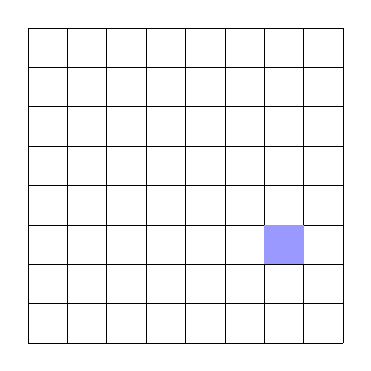
\begin{tikzpicture}
    \draw[step=0.5cm,black,very thin] (-2,-2) grid (2,2);
    \fill[blue!40!white] (1,-1) rectangle (1.5,-0.5);
  \end{tikzpicture}
\end{center}
Two people look at this board and decide to play a game. \\
One tells the other ``Let's take turns moving this knight towards the top left
of this board using only knight-like moves. If I am left with no
legal moves on my turn, I lose. If you can't make any move on your
turn, you lose'', and since she is bored, she readily agrees. \\
What can we say about this game? For clarity, the moves that the first
player can make are highlighted in red below. The the possible moves
for the rest of the game should be clear $\ldots$
\begin{center}
  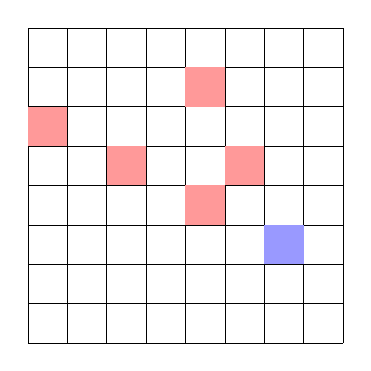
\begin{tikzpicture}
    \draw[step=0.5cm,black,very thin] (-2,-2) grid (2,2);
    \fill[blue!40!white] (1,-1) rectangle (1.5,-0.5);
    \fill[red!40!white] (0.5,0) rectangle (1,0.5);
    \fill[red!40!white] (0,1) rectangle (0.5,1.5);
    \fill[red!40!white] (0,-0.5) rectangle (0.5,0);
    \fill[red!40!white] (-1,0) rectangle (-0.5,0.5);
    \fill[red!40!white] (-2,0.5) rectangle (-1.5,1);
  \end{tikzpicture}
\end{center}
Note that the term ``\SUDL{} move'' means a move where the knight moves
$i$ squares above and $2i$ squares to the left. What this $i$ will
be understood easily from the context of the explanation. \\
Similarly the term ``\DUSL{} move'' means a move where the knight moves
$2i$ squares above and $i$ squares to the left. What this $i$ will
be understood easily from the context of the explanation. \\
Observe that every square has a certain nimber, so \textit{ideally} we
should come up with a system to figure out the nimber given a
row, column pair. \\
For additional inspiration/motivation, a manually computed and 
color-coded diagram of the board is presented below:
\begin{center}
  \includegraphics[scale=0.2]{chessboardWithNimbers}
\end{center}
\newpage

This is a larger, uncolored version of the board with more nimbers. There are
26 rows and 26 colums.
\begin{center}
  \includegraphics[scale=0.5]{expandedchessboard}
\end{center}
\newpage

\paragraph{Chess Analysis}\mbox{}\\
First we establish a numbering for all the squares. \\
A square can be identified by a (row, column) pair. \\
The rows are numbered from top to bottom, starting at $0$. \\
The columns are numbered from left to right, also starting at $0$.
\medskip

Let $\D{(r,c)}{m}$ represent the square $(r + m, c + 2m)$, where
$r$, $c$ and $m$ can come from the set $\N \cup \{0\}$.
\medskip

Now that this has been established we can proceed to prove
some claims.

\begin{claim}
\begin{equation*}
  \nim(\D{(0,i)}{m}) = m,\ \T{for any}\ i \geq 0
\end{equation*}
\end{claim}

\begin{claimproof}\mbox{}\\
We will use strong induction.
\medskip

\I{Base Cases:} \\
$\nim(\D{(0,i)}{0}) = 0$ \\
$\nim(\D{(0,i)}{1}) = 1$ \\
The values for the base cases can be read off the
figure on the previous page.
\medskip

\I{Induction Hypothesis:} \\
Suppose for some $m \in \N$, the claim is true for all $k < m$.
\medskip

\I{Induction Step:} \\
We want to prove that the claim is true for $m + 1$.
\smallskip

Consider the square $\D{(0,i)}{m+1}$, and notice that
we can reach any square of the form $\D{(0,i)}{i}$ where
$0 \leq i \leq m$ from this square using a single-up double-left
move. 
So by the I.H., we can reach any position with nimber $i$ where
$0 \leq i \leq m$ from the square using a single-up double-left
move.
\smallskip

Now consider an arbitrary square reachable from $\D{(0,i)}{m+1}$
with a double-up single-left move. We can only make \I{less than}
$m+1$ single-up double-left or \I{less than} $m+1$ double-up single-left
moves from such a square to reach the sides of the square, so
it is just not possible for such a square to have a nimber
greater than or equal to $m+1$.
\smallskip

Thus, the set of nimbers of all the positions reachable from
$\D{(0,i)}{m+1}$ is just $\{0,1,2,\ldots,m\}$. By the
Sprague-Grundy Theorem, $\nim(\D{(0,i)}{m+1}) = m+1$ because
$m+1 = \T{mex}(\{0,1,2,\ldots,m\})$.
\smallskip

Thus the claim is true for $m+1$.
\end{claimproof}
\newpage

\begin{claim}
\begin{equation*}
  \nim(\D{(2,1)}{m}) =
  \begin{cases}
    \, (m+1), \ \T{if}\ m \equiv 0 \pmod{2} \\
    \, (m-1), \ \T{if}\ m \equiv 1 \pmod{2}
  \end{cases}
\end{equation*}
\end{claim}

\begin{claimproof}\mbox{}\\
We will use a variant of strong induction.
\medskip

\I{Base Cases:} \\
$\nim(\D{(2,1)}{0}) = 1$ \\
$\nim(\D{(2,1)}{1}) = 0$ \\
$\nim(\D{(2,1)}{2}) = 3$ \\
$\nim(\D{(2,1)}{3}) = 2$ \\
The values for the base cases can be read off the
figure on the previous page.
\medskip

\I{Induction Hypothesis:} \\
Suppose for some $m \in \N$, $m \equiv 1 \pmod{2}$
the claim is true for all $k < m$.
\medskip

\I{Induction Step:} \\
We want to prove that the claim is true for $m + 1$ and $m + 2$.
\medskip

We need to prove that 
$\nim(\D{(2,1)}{m+1}) = m + 2$. \\
From $\D{(2,1)}{m+1}$, we can reach any square of the form
$\D{(2,1)}{2j}$ where $0 \leq j \leq \frac{m+1}{2}-1$ 
using a \SUDL{} move. \\
By the induction hypothesis,
this means that from $\D{(2,1)}{m+1}$ we can reach squares
with nimbers in \\ 
the set $\{2j+1 : 0 \leq j \leq \frac{m-1}{2}\} =$
$\{o : o\ \T{is an odd number less than}\ m+1\}$. \\
From $\D{(2,1)}{m+1}$, we can also reach any square of the form
$\D{(2,1)}{2j+1}$ where $0 \leq j \leq \frac{m-1}{2}$
using a \SUDL{} move. \\
this means that from $\D{(2,1)}{m+1}$ we can reach squares
with nimbers in \\ 
the set $\{2j : 0 \leq j \leq \frac{m-1}{2}\} =$
$\{e : e\ \T{is an even number less than}\ m+1\}$. \\
It follows that from $\D{(2,1)}{m+1}$, we can definitely
reach game states with nimbers in the set $\{0,1,\ldots,m\}$. \\
Now consider an arbitrary square reachable from $\D{(2,1)}{m+1}$
with a double-up single-left move. We can only make \I{less than}
$m+1$ single-up double-left or \I{less than} $m+1$ double-up single-left
moves from such a square to reach the sides of the square, so
it is just not possible for such a square to have a nimber
greater than $m+1$. \\
But notice that when we start out at $\D{(2,1)}{m+1}$ and then
move two squares up and one square to the left we get
to the square $\D{(0,0)}{m+1}$, whose nimber --- as we proved
earlier --- is $m+1$. \\
No other squares reachable from $\D{(2,1)}{m+1}$ matter to us as
they have lower nimbers. \\
We have shown that from this square we can get to game states
whose nimbers cover the set $\{0,1,\ldots,m+1\}$. \\
By the Sprague-Grundy Theorem, 
$\nim(\D{(2,1)}{m+1}) = \T{mex}(\{0,1,\ldots,m+1\}) = m + 2$. \\
This means that the claim holds for $m+2$.
\medskip

Now consider the square $\D{(2,1)}{m+2}$. \\
We want to show $\nim(\D{(2,1)}{m+2}) = m+1$. \\
We already know that using \SUDL{} moves from $\D{(2,1)}{m+2}$,
the nimbers of the game states that we can reach cover the set
$(\{0,1,\ldots,m+2\} \setminus \{m+1\})$. \\
Notice that $\D{(2,1)}{m+2} = (m+4,2m+5)$. \\
If we move two squares up and one square left from here we reach
$(m+2, 2m+4) = \D{(0,0)}{m+2}$ which has nimber $m+2$. \\
If we move another two squares up and one square left we get to
$(m, 2m+3) = \D{(0,3)}{m}$, which has nimber $m$. \\
Moving a further two squares up and one square left takes us to
$(m-2, 2m+2)$. Note that from here the number of possible
\SUDL{} moves is $m-2$ and the number of \DUSL{} moves is 
$\frac{m-2}{2}$, so this square has a nimber that is less 
than or equal to $m-1$. \\
Thus all the other moves of the \DUSL{} variety are irrelevant
to us. \\
It follows that the set of the nimbers of all the squares that we
can reach from $\D{(2,1)}{m+2}$ is
$(\{0,1,\ldots,m+2\} \setminus \{m+1\})$. The mex of this set is
$m+1$, so by the Sprague-Grundy Theorem,
$\nim(\D{(2,1)}{m+2}) = m+1$.
\medskip

We have proved that the claim holds for $m+1$ and $m+2$.
\end{claimproof}
\newpage

\begin{claim}
\begin{equation*}
  \nim(\D{(3,0)}{m}) =
  \begin{cases}
    \, m,  &\ \T{if}\ m \equiv 0   \pmod{4} \\
    \, m+1,&\ \T{if}\ m \equiv 1,2 \pmod{4} \\
    \, m-2,&\ \T{if}\ m \equiv 3   \pmod{4} \\
  \end{cases}
\end{equation*}
\end{claim}

\begin{claimproof}\mbox{}\\
We will use a variant of strong induction.
\medskip

\I{Base Cases:} \\
$\nim(\D{(3,0)}{0}) = 0$ \\
$\nim(\D{(3,0)}{1}) = 2$ \\
$\nim(\D{(3,0)}{2}) = 3$ \\
$\nim(\D{(3,0)}{3}) = 1$ \\
$\nim(\D{(3,0)}{4}) = 4$ \\
$\nim(\D{(3,0)}{5}) = 6$ \\
$\nim(\D{(3,0)}{6}) = 7$ \\
$\nim(\D{(3,0)}{7}) = 5$ \\
The values for the base cases can be read off the
figure on the previous page.
\medskip

\I{Induction Hypothesis:} \\
Suppose for some $m \in \N$, $m \equiv 3 \pmod{4}$
the claim is true for all $k < m$.
\medskip

\I{Induction Step:} \\
We want to prove that the claim is true for $m + 1$, $m + 2$,
$m + 3$ and $m + 4$.
\medskip

First consider 
\end{claimproof}
\newpage

\paragraph{Chess Possibilities}\mbox{}\\
The observation that we can make by looking at the nimbers
(using a program to calculate nimbers) is that the values
of $\D{(r,c)}{m+1}-\D{(r,c)}{m}$ for $m \geq 0$ may initially
appear to be unstructured and then settle into a cycle,
repeating periodically. Also, there is a different cycle for
each new initial $(r,c)$ used as a starting point for
$\D{(r,c)}{m}$.
\bigskip

Some cycles that have been observed (but not proved) follow. They have
been matched up with the appropriate starting squares in (row, column)
notation. Keep in mind that some of sequences start with seemingly
unpredictable nimbers and those parts have been disregarded.
\begin{verbatim}
(7 , 7):  5, 1, 1,-3
(8 , 8):  5, 1, 1,-3, 4, 2, 1, 1,-3
(9 , 9):  2, 1,-2, 3 
(10,10):  6, 1, 1, 1,-4, 6, 1, 1, 1,-4, 5, 2, 1, 1, 1,-4 
(11,11): -1,-2, 5, 1, 2,-4, 6, 1,-4, 6,-4, 5, 1,-3, 6,-1, 
          2,-3, 4, 3, 1, 1,-4, 1, 4, 2, 2 
(12,12):  1, 1,-5, 7, 1, 1 
(13,13):  7, 1,-5, 6, 1,-4, 7, 1, 1, 1,-5, 1, 5, 3, 1, 1,
          1,-5, 1, 6, 1, 2, 1,-5, 7, 1,-5, 7,-1,-3, 6, 2,
         -1, 3,-5, 6, 1, 2,-5, 7,-1, 2,-4, 7,-1, 3, 1,-5
(14,14):  1, 1, 1,-4, 6,-1, 2, 2,-1, 3, 1, 1, 1,-4, 6, 1, 
          1, 1,-4, 5, 1, 2, 1, 1, 1,-4, 6
(15,15):  1, 1,-6, 1, 8, 1, 1, 1, 1,-6, 1, 8, 1, 1, 1, 1,
         -6, 1, 8, 1, 1, 1, 1,-6, 1, 7, 2, 1, 1, 1,-6, 7,
         -5, 8, 1, 1 
\end{verbatim}
\bigskip

The idea is that these can lead us to new formulae worth proving
(like the ones proved in the analysis section).
\end{document}
